\documentclass[letterpaper]{report}
%\usepackage[utf8]{inputenc}
\usepackage[T1]{fontenc}
\usepackage{RJournal}
\usepackage{amsmath,amssymb,array}
\usepackage{booktabs}

%% load any required packages here

\usepackage[spanish]{babel}
\usepackage{graphicx}

\hypersetup{pdftitle={MinaR los discuRsos pResidenciales},
            pdfkeywords={discurso; text minning; política}}



\hypersetup{pdfauthor=Anónimo}


%\usepackage[hidelinks]{hyperref}

\urlstyle{same}  % don't use monospace font for urls
\usepackage{color}
\usepackage{fancyvrb}
\newcommand{\VerbBar}{|}
\newcommand{\VERB}{\Verb[commandchars=\\\{\}]}
\DefineVerbatimEnvironment{Highlighting}{Verbatim}{commandchars=\\\{\}} 
% Add ',fontsize=\small' for more characters per line
\usepackage{framed}
\definecolor{shadecolor}{RGB}{248,248,248}
\newenvironment{Shaded}{\begin{snugshade}}{\end{snugshade}}
\newcommand{\AlertTok}[1]{\textcolor[rgb]{0.94,0.16,0.16}{#1}}
\newcommand{\AnnotationTok}[1]{\textcolor[rgb]{0.56,0.35,0.01}{\textbf{\textit{#1}}}}
\newcommand{\AttributeTok}[1]{\textcolor[rgb]{0.77,0.63,0.00}{#1}}
\newcommand{\BaseNTok}[1]{\textcolor[rgb]{0.00,0.00,0.81}{#1}}
\newcommand{\BuiltInTok}[1]{#1}
\newcommand{\CharTok}[1]{\textcolor[rgb]{0.31,0.60,0.02}{#1}}
\newcommand{\CommentTok}[1]{\textcolor[rgb]{0.56,0.35,0.01}{\textit{#1}}}
\newcommand{\CommentVarTok}[1]{\textcolor[rgb]{0.56,0.35,0.01}{\textbf{\textit{#1}}}}
\newcommand{\ConstantTok}[1]{\textcolor[rgb]{0.00,0.00,0.00}{#1}}
\newcommand{\ControlFlowTok}[1]{\textcolor[rgb]{0.13,0.29,0.53}{\textbf{#1}}}
\newcommand{\DataTypeTok}[1]{\textcolor[rgb]{0.13,0.29,0.53}{#1}}
\newcommand{\DecValTok}[1]{\textcolor[rgb]{0.00,0.00,0.81}{#1}}
\newcommand{\DocumentationTok}[1]{\textcolor[rgb]{0.56,0.35,0.01}{\textbf{\textit{#1}}}}
\newcommand{\ErrorTok}[1]{\textcolor[rgb]{0.64,0.00,0.00}{\textbf{#1}}}
\newcommand{\ExtensionTok}[1]{#1}
\newcommand{\FloatTok}[1]{\textcolor[rgb]{0.00,0.00,0.81}{#1}}
\newcommand{\FunctionTok}[1]{\textcolor[rgb]{0.00,0.00,0.00}{#1}}
\newcommand{\ImportTok}[1]{#1}
\newcommand{\InformationTok}[1]{\textcolor[rgb]{0.56,0.35,0.01}{\textbf{\textit{#1}}}}
\newcommand{\KeywordTok}[1]{\textcolor[rgb]{0.13,0.29,0.53}{\textbf{#1}}}
\newcommand{\NormalTok}[1]{#1}
\newcommand{\OperatorTok}[1]{\textcolor[rgb]{0.81,0.36,0.00}{\textbf{#1}}}
\newcommand{\OtherTok}[1]{\textcolor[rgb]{0.56,0.35,0.01}{#1}}
\newcommand{\PreprocessorTok}[1]{\textcolor[rgb]{0.56,0.35,0.01}{\textit{#1}}}
\newcommand{\RegionMarkerTok}[1]{#1}
\newcommand{\SpecialCharTok}[1]{\textcolor[rgb]{0.00,0.00,0.00}{#1}}
\newcommand{\SpecialStringTok}[1]{\textcolor[rgb]{0.31,0.60,0.02}{#1}}
\newcommand{\StringTok}[1]{\textcolor[rgb]{0.31,0.60,0.02}{#1}}
\newcommand{\VariableTok}[1]{\textcolor[rgb]{0.00,0.00,0.00}{#1}}
\newcommand{\VerbatimStringTok}[1]{\textcolor[rgb]{0.31,0.60,0.02}{#1}}
\newcommand{\WarningTok}[1]{\textcolor[rgb]{0.56,0.35,0.01}{\textbf{\textit{#1}}}}

\providecommand{\keywords}[1]{\noindent\textbf{Palabras clave:} #1}
\providecommand{\tightlist}{%
\setlength{\itemsep}{0pt}\setlength{\parskip}{0pt}}


\begin{document}

%% do not edit, for illustration only
\sectionhead{MinaR los discuRsos pResidenciales}
\year{2020}

\begin{article}

\title{MinaR los discuRsos pResidenciales}


\author{Anónimo}

\maketitle


\keywords{ discurso  -  text minning  -  política }

\hypertarget{abstract}{%
\section{Abstract}\label{abstract}}

El primero de marzo de cada año las cámaras de Diputados y Senadores de
la Nación Argentina se reúnen en asamblea para dar comienzo al año
legislativo. Cada año el presidente de turno encabeza dicho acto con un
discurso\footnote{La fuente original de todos los discursos puede
  consultarse en línea en
  \url{https://www.hcdn.gob.ar/secparl/dgral_info_parlamentaria/dip/documentos/mensajes_presidenciales.html}}.
Éstos suelen girar en torno a los ejes de gobierno o promesas y
objetivos del año. Es notorio que estos mensajes tiene un estilo y
contenido marcado por quien ejerce el gobierno. En este trabajo partimos
de una gran cantidad de texto contenido en cada uno de los discursos
presidenciales desde el retorno de la democracia en 1983 para poder
encontrar tanto patrones comunes como diferencias entre los mandatarios
a lo largo del tiempo.

Hacer uso de la \emph{minería de texto} de los discursos de los
presidentes como estrategia de investigación es de utilidad para un
rápido y eficiente análisis exploratorio del gran volúmen de información
contenida en los mismos. Dentro del ecosistema de \texttt{R} este campo
ha ido creciendo sostenidamente. Liberias como \CRANpkg{tm} y
\CRANpkg{topicmodels} son herramientas poderosas para el procesamiento,
manipulación y modelado de la información contenida en el texto.
Siguiendo la filosofía de \CRANpkg{tidyverse} Sigle y Robinson (2016)
desarrollaron \CRANpkg{tidytext}, que hace mucho más facil una primera
introducción a esta técnica de investigación y su integración con otras
como \CRANpkg{ggplot2} para la visualización.

Un flujo de trabajo como el descripto más arriba puede ilustrarse
siguiendo el esquema propuesto por Silge y Robinson (2020):

\begin{center}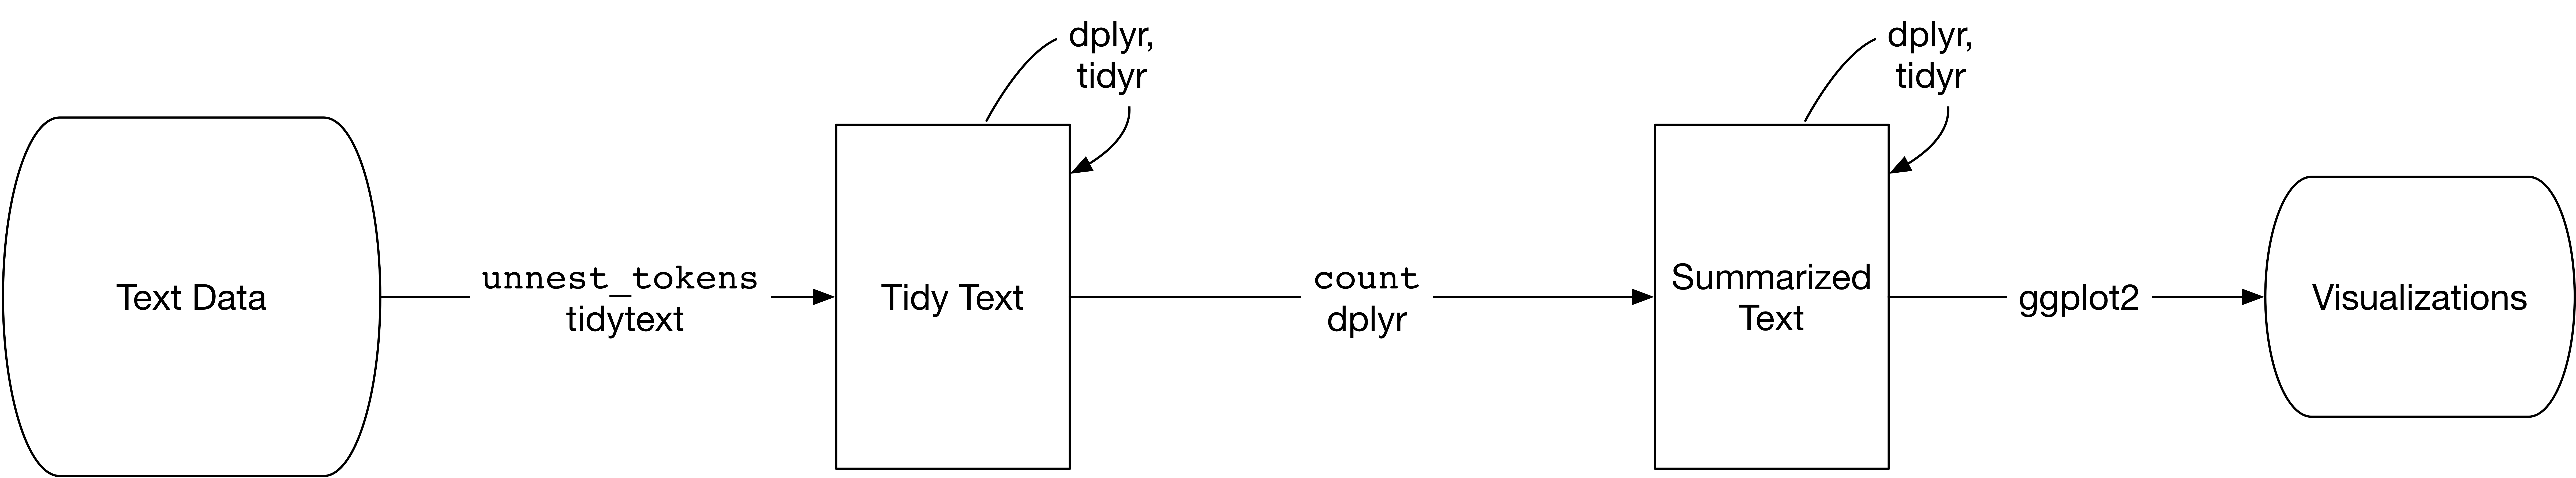
\includegraphics[width=0.8\linewidth]{../../img/diagrama} \end{center}

\begin{enumerate}
\def\labelenumi{\arabic{enumi}.}
\item
  Descargamos los archivos con el texto de \(37\) discursos emitidos por
  \(8\) presidentes. Desde el primero de Alfonsín en la transición a la
  democracia (1984) hasta el último con el que Alberto Fernández dio
  inicio a las sesiones legislativas (2020). Entre todos suman alrededor
  de \(365_{mil}\) palabras con un promedio de \(9.880\) y picos mínimo
  de \(2.846\) (Carlos Menem en 1996) y máximo de \(26.189\) (Cristina
  Fernández de Kirchner en \(2013\)).
\item
  Con esa información construimos una única base de datos siguiendo el
  principo \emph{datos de texto ordenados} (\emph{tidy text}) propuesto
  por Sigle y Robinson (2016) como extensión de los \emph{datos
  ordenados} (\emph{tidy}) de Wickham (2014):
\end{enumerate}

\begin{itemize}
\tightlist
\item
  Cada variable debe tener su propia columna.
\item
  Cada observación debe tener su propia fila.
\item
  Cada valor debe tener su propia celda.
\end{itemize}

Sigle y Robinson (2016) definen entonces a los \emph{datos de texto
ordenados} cuando están en una tabla compuesta por ``un \emph{token} por
fila''. \emph{Un token es una unidad de texto significativa, como una
palabra} (o un \emph{bigrama})\emph{, que estamos interesados en usar
para el análisis, y la tokenización es el proceso de dividir el texto en
tokens}\footnote{Traducción propia de \emph{The tidy text format} (Silge
  and Robinson 2016).}.

\begin{enumerate}
\def\labelenumi{\arabic{enumi}.}
\setcounter{enumi}{2}
\tightlist
\item
  Trabajamos con \CRANpkg{dplyr} para calcular frecuencias de palabras y
  \CRANpkg{tidytext} para calcular palabras de mayor importancia
  comparada entre discursos (\emph{tf\_idf}). Por último
  \CRANpkg{ggplot2} (y extensiones como \CRANpkg{patchwork} y
  \CRANpkg{ggforce}) para las visualizaciones.
\end{enumerate}

\hypertarget{ejemplo-primeros-discursos-presidenciales}{%
\subsection{Ejemplo: primeros discursos
presidenciales}\label{ejemplo-primeros-discursos-presidenciales}}

Inspirados en un trabajo del equipo de datos de la Universidad de
Berkeley (California)\footnote{\emph{The Language of Data: Analyzing the
  State of the Union} (datascience@berkeley 2019).} calculamos la
frecuencia con la que los presidentes utilizaron determinadas palabras
relacionadas con un tópico específico, en este caso etiquetadas como
\emph{Política}.

\begin{center}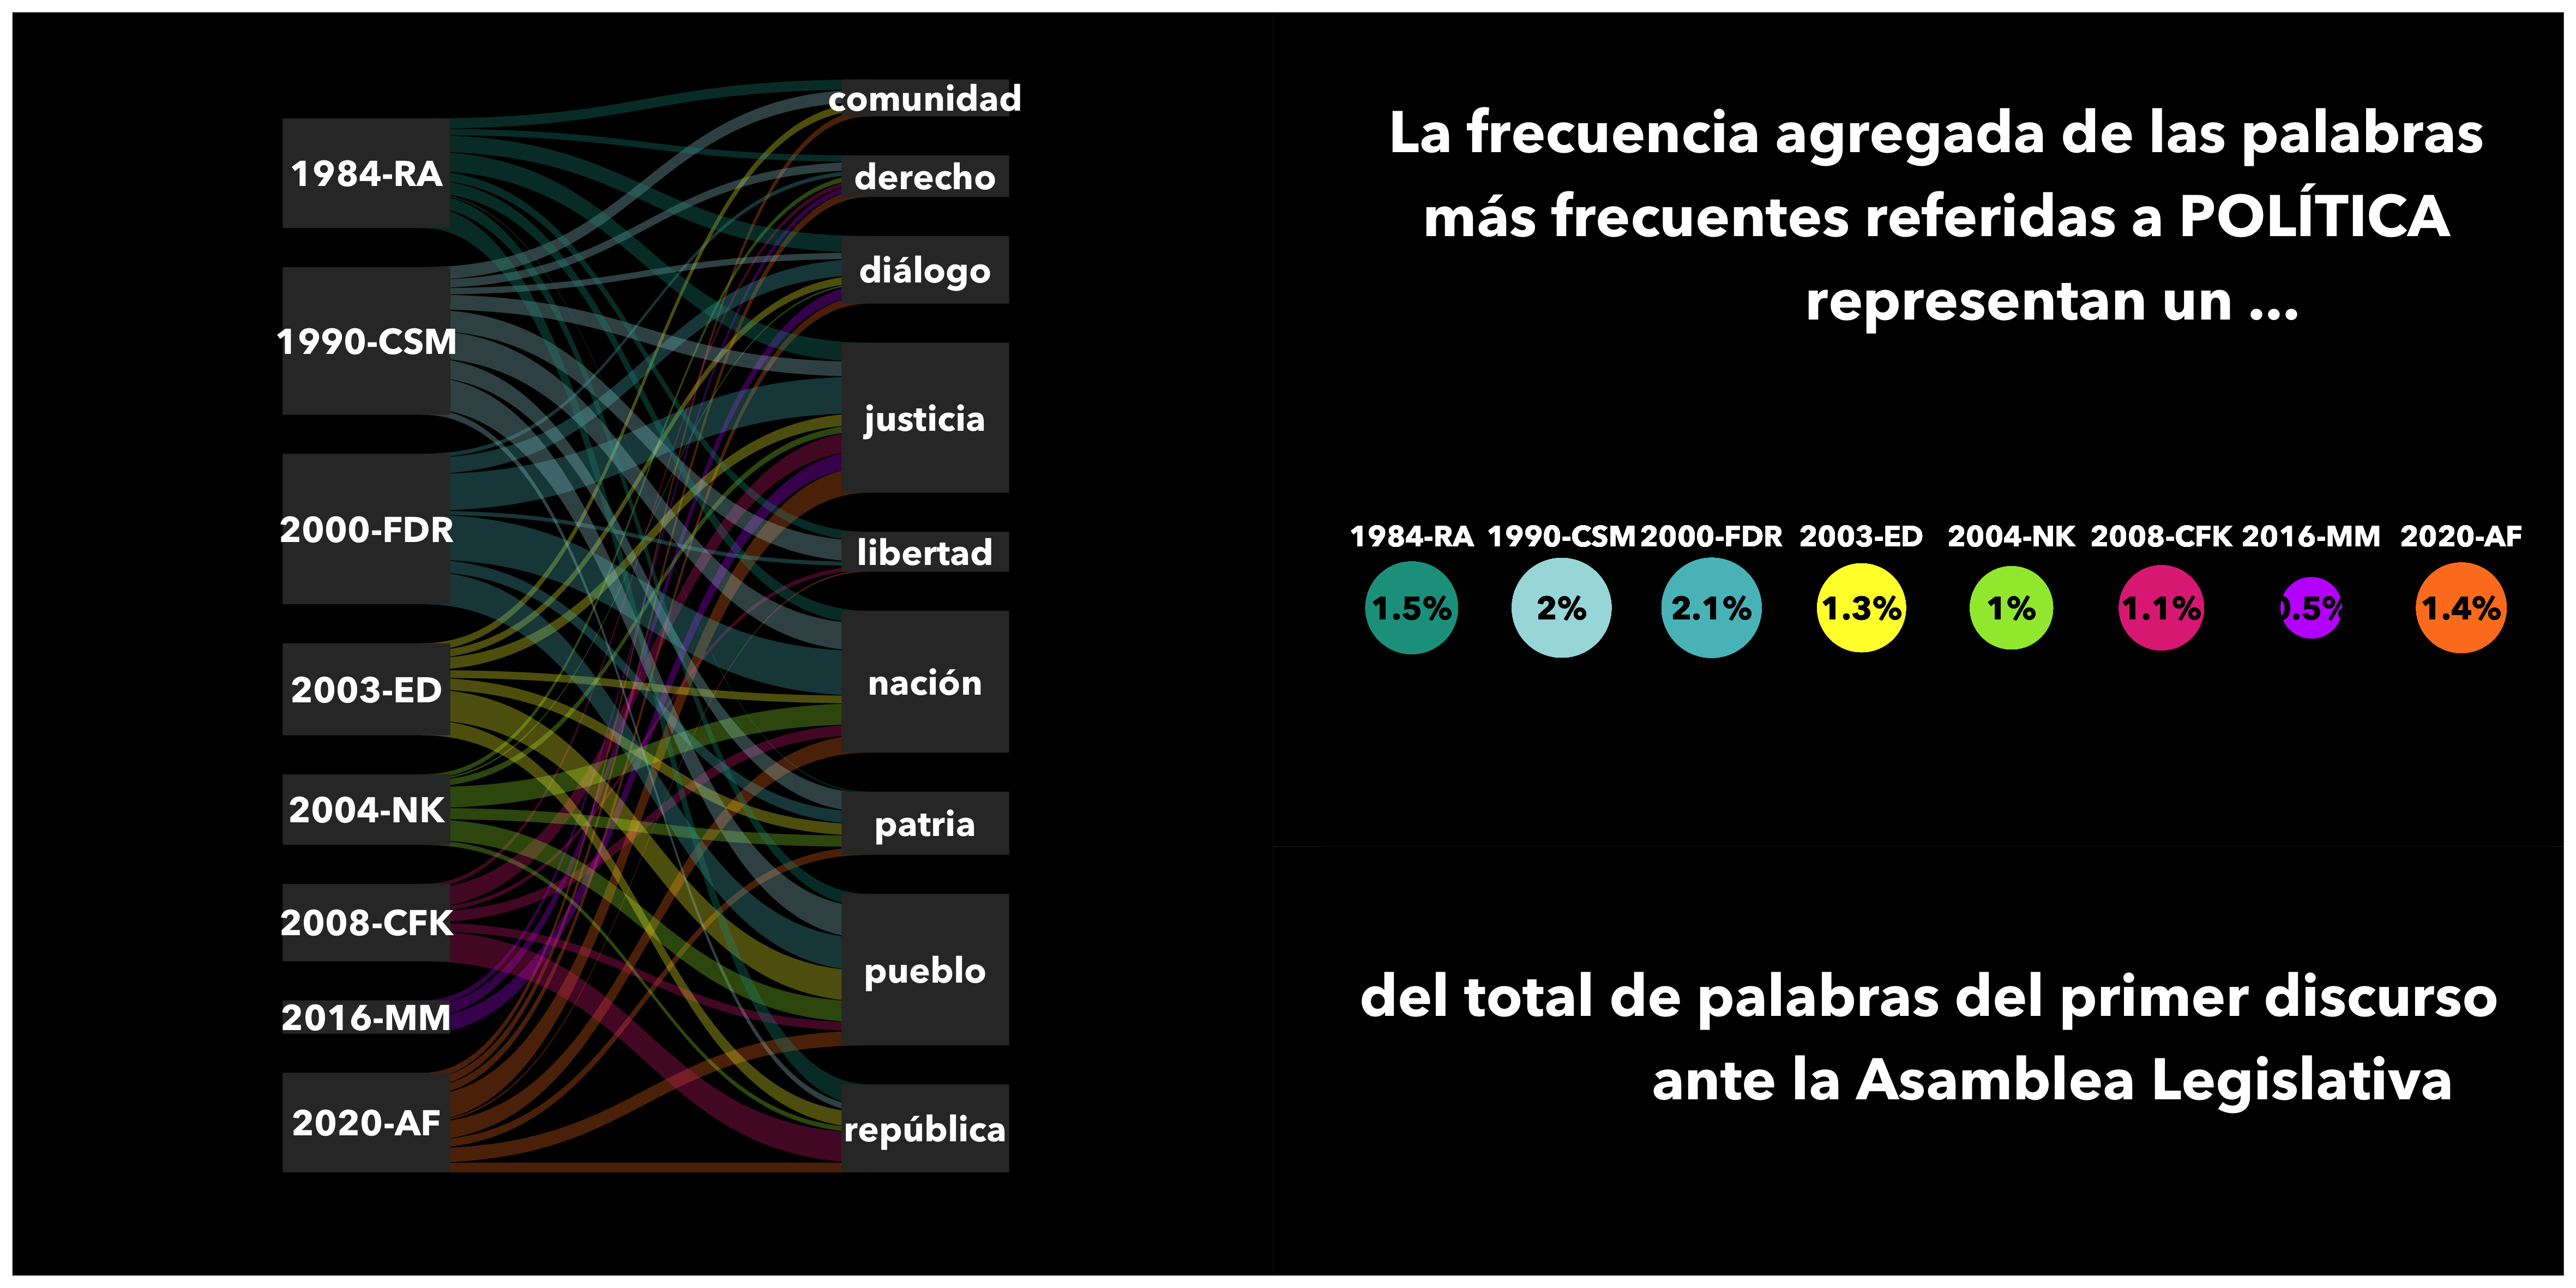
\includegraphics[width=1\linewidth]{../../img/parallel_dot2} \end{center}

\hypertarget{referencias}{%
\section*{Referencias}\label{referencias}}
\addcontentsline{toc}{section}{Referencias}

\hypertarget{refs}{}
\leavevmode\hypertarget{ref-berkeley}{}%
datascience@berkeley. 2019. ``The Language of Data: Analyzing the State
of the Union,'' January.
\url{https://datascience.berkeley.edu/blog/trump-state-of-the-union-analysis/}.

\leavevmode\hypertarget{ref-Silge2016}{}%
Silge, Julia, and David Robinson. 2016. ``Tidytext: Text Mining and
Analysis Using Tidy Data Principles in R.'' \emph{Journal of Open Source
Software} 1 (3). The Open Journal: 37.
\url{https://doi.org/10.21105/joss.00037}.

\leavevmode\hypertarget{ref-silge_text_2020}{}%
---------. 2020. \emph{Text Mining with R}. O'Reilly.
\url{https://www.tidytextmining.com/}.

\leavevmode\hypertarget{ref-JSSv059i10}{}%
Wickham, Hadley. 2014. ``Tidy Data.'' \emph{Journal of Statistical
Software, Articles} 59 (10): 1--23.
\url{https://doi.org/10.18637/jss.v059.i10}.




\end{article}
\end{document}

